\chapter{Реализация программного комплекса NA64}

Данная глава посвящена описанию реализации
программного комплекса и соответствующим физическим результатам,
полученным с применением описанных ранее методов.

\begin{comment}
Реконструкция данных представляет собой преобразование
сигналов детекторов в рамках одной и той же согласованной модели,
с применением калибровочной информации.

Применение конкурирующих численных методов и их динамическая композиция
могут быть обобщены в рамках машины конечных состояний, которые применяются,
в частности, к задаче аппроксимации амплитудной функции сигналов калориметров
или реконструкции треков с проверкой конкурирующих гипотез.

С практической точки зрения, многие элементарные
варианты использования могут быть эффективно обобщены
в рамках специализированных выразительных средств (искусственных
языков). В частности, они обеспечивают мощные
выразительные средства для повторяющихся задач:
выбор детекторов, запросы к модели события, описание калибровочных
данных.

Выбор форматов данных должен быть обоснован в рамках заданных
архитектурных инвариантов, фиксируя протоколы обмена данными между
основными компонентами.
\end{comment}

%В главе рассмотрены реализации компонент программного комплекса,
%выполняющих конкретные задачи в рамках предложенной архитектурной
%концепции. Глава завершается изложением физических результатов
%полученных с применением этих средств.

\section{Динамические машины состояний}

Для решения задач выбора конкурирующих гипотез -- таких, как разделение
амплитудных импульсов во времени или выбор между гипотезами о
треке частицы,
%в рамках подхода быстрого прототипирования,
целесообразно прибегнуть к высокому уровню общности,
поскольку по мере появления новых детекторов и считывающей аппаратуры,
тестирования и разработки новых методов реконструкции сигналов,
необходимо производить исследование поведения существующих алгоритмов,
производить оптимизацию параметров и часто изменять систему.

Истинная функция отклика подвержена влиянию многих факторов: существенно
зависит от считывающей аппаратуры и изменяется в зависимости от вещества
рабочего объёма детектора.
%Используемая в качестве приближения
%\emph{модельная функция} $f(t,\vec{p})$ --- аппроксимация амплитуды в момент
%времени $t$ праметризуемая параметрами $\vec{p}$
С некоторыми допущениями, для реконструкции
можно применять упрощённую модель или быстрый алгоритм реконструкции с
потерей точности там, где ошибки не так важны как средняя картина
наблюдаемых распределений -- например, при
мониторировании детекторов во время набора данных.
Напротив, для задач анализа целесообразно
стремиться к наиболее правдоподобной модели -- например, для улучшения
разрешения при реконструкции ливней в калориметрах, поскольку
малые амплитуды на периферии ливня приобретают большое значение
в дискриминационных логических схемах.

%Важно отметить, что помимо задачи
%разрешения откликов САЦП, общая постановка задачи справедлива и для
%задачи реконструкции треков, которая в общем формулируется чаще всего
Например, задача реконструкции треков формулируется
как задача минимизации функционала статистики
$\chi^2 = \sum\limits_i (f((t_i,\vec{p}) - r_i)/\sigma_i)^2$ от некоторой (в
общем -- нелинейной, необязательно аналитической) функции параметризации
трека $f(t,\vec{p})$ по отношению к выбранным наборам показаний
координатно-чувствительных детекторов $\vec{r}_i$. При этом
%, как правило, при больших загрузках детекторов,
%типичных для современных экспериментов с большой светимостью,
для разрешения возникающих неоднозначностей применяются различные
алгоритмы отбора: в рамках общей задачи поиска трека~(\emph{track finding})
поиск может производиться по известным пространственным
шаблонам~(\emph{pre-patterning}),
на основе пространственных биекций,
разбиения на KD-дерево, и т.д. ~\cite{MankelTracking, artificial-retina-tracking-lhc}
Такие алгоритмы обычно дают довольно грубое
приближение для более высокоуровневого алгоритма аппроксимации трека,
существенно снижающее набор входных значений по отношению к прямому
комбинаторному перебору.

\subsection{Варианты использования}

Будем подразумевать под \emph{моделью} математическую
функцию $f(x,\vec{p})$, определённую в зависимости от некоторого
аргумента $x_i$ и вектора параметров $\vec{p}$. Целью
\emph{процедуры минимизации} является отыскание таких параметров $\vec{p}$
при которых достигается наилучшее соответствие набору входных данных $y_i$
согласно некоторой метрике.
При этом под программной~\emph{процедурой} в общем, далее мы будем понимать формальный
алгоритм осуществляющий преобразование вектора параметров
модели~$P(\vec{p}_a) = \vec{p}_b$ (т.е. не обязательно
минимизации).
%Символически, можно записать, что для некоторой метрики $\mathbb{M}$
%преобразование заданное процедурой $P$
%т.е. целью процедуры как преобразования $P[\vec{p}_a] \rightarrow \vec{p}_b$
%является отыскание таких $\vec{p}_b$ при которых достигается
%условие~$\text{min}()$

Выделим как минимум следующие основные варианты использования системы,
с точки зрения пользовательского кода, расширяющие исходный
сценарий~\emph{применения процедуры к программной модели}:
\begin{itemize}
    \item Элементарный вариант использования состоит в прямом
    \emph{изменении параметров модельной функции}. Такой этап может быть
    полезен, например, при введении искусственного возмущения в
    линейных алгоритмах минимизации с целью преодоления локальных
    минимумов.
    \item \emph{Применения алгоритма численной минимизации}. Помимо МНК сюда
    относится, например, фильтр Калмана в его различных модификациях,
    и в целом задачи линейного программирования допускающие выражение
    в виде линейно-алгебраических операций над модельной функцией с
    фиксированным набором параметров.
    \item Выбор и \emph{установка начальных значений} параметров $\vec{p}$
    на основе исходной выборки значений $x_i$. Этот вариант
    подразумевает предварительной вычисление начальных приближений
    на основе широкого набора параметров регулирующих поведение
    поисковых алгоритмов.
    \item \emph{Применение процедур к отдельным элементам и подразумеваемая}
    в таком случае \emph{декомпозицию модели} может понадобиться,
    когда с точки зрения численной процедуры минимизации, модель может
    быть тем или иным образом разложена (факторизована) на набор более
    элементарных независимых моделей, к каждой из которых необходимо
    применить определённый набор процедур. Например: аппроксимация
    функции отклика для значительно разнесённых во времени пиков,
    аппроксимация трека частицы на линейных участках в отсутствии
    магнитного поля, и т.д.
    \item Для \emph{сопоставления результатов} аппроксимации между
    конкурентными методами посредством определённой метрики (в частности,
    выбор наилучшей гипотезы о треке на основании $\chi^2$), необходима
    соответствующая процедура, делегирующая выполнение альтернативным процедурам.
    \item В тех случаях, когда метрика не может быть определена для
    моделей, и основным результатом является логическое условие применимости
    процедуры, целесообразно выделить вариант использования перебирающий
    процедуры до тех пор, пока очередной вариант не будет
    выполнен успешно (\emph{выбор подходящей модели}).
    \item Наконец, \emph{выбор или замена модельной функции} в рамках
    такого уровня общности тоже представляет собой вариант использования.
\end{itemize}

\begin{figure}
    \centering
    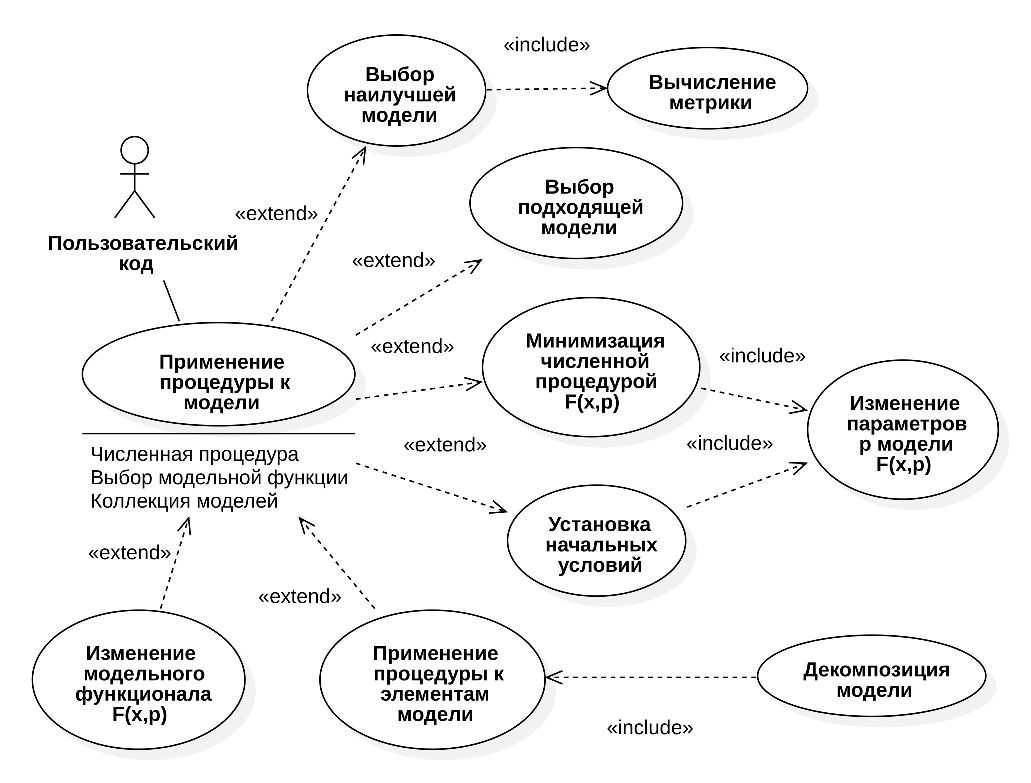
\includegraphics[width=0.95\linewidth]{images/umff-usecase-diagram-02.eps}
    \caption{Диаграмма вариантов использования программной библиотеки для
    решения задач численной минимизации с расширенной логикой (ветвление,
    сопоставление, перебор).}
    \label{fig:umff-usecases}
\end{figure}

Рисунок \ref{fig:umff-usecases} иллюстрирует отношения между перечисленными вариантами
использования.

\subsection{Компоненты машины конечных состояний}

Описанная структура вариантов использования подразумевает наличие по крайней мере
следующих элементов обобщённого поведения:
\begin{itemize}
    \item Составная процедура содержащая набор более простых процедур,
    делегирующая выполнение этому набору, и завершающаяся результатом
    отобранным согласно некоторому правилу (\emph{competing}).
    \item Составная процедура осуществляющая декомпозицию модели в тех случаях,
    когда модель это позволяет, инкапсулирующая набор более простых процедур,
    и применяющая этот набор по отдельности к каждому элементу
    декомпозиции~(\emph{breakdown}).
    \item Последовательность процедур в которой последующая применяется только
    в том случае, если текущая завершилась не успешно
    (\emph{fallback}).
    %Рисунок \ref{fig:fallback-example} содержит
    %пример машины конечных состояний, в которой применение процедуры
    %делегируется, а валидация выполняется самим элементом.
\end{itemize}

Этот базовый набор логических элементов позволяет конструировать сложные
алгоритмы, опираясь на более элементарные, порождая машину
конечных состояний, в которой состояниям отвечает модель ($m_i:=f(x_i,\vec{p})$),
а переходам соответствует процедура $P(\vec{p}_a) = \vec{p_b}$.

Техническое описание и спецификации вынесены в приложение~\ref{appendix:fsm-machine-prog}.

\subsection{Восстановление амплитудных сигналов}

На рисунке~\ref{fig:sadc-wf-fitting-example} приведён пример
восстановленного отклика ячейки электромагнитного калориметра от двух
импульсов слабо разнесённых во времени. Пунктирной линией
с коротким штрихом
изображён график конечно-разностной аппроксимации первой производной
по точкам сигнала, сплошными серыми линиями изображён результат
подгонки -- для отдельных импульсов и их восстановленная сумма.
Пунктирная линия с длинным штрихом отвечает начальным условиям.

\begin{figure}[ht]
    \centering
    \includegraphics[width=0.99\linewidth]{images//illustrative/waveform-fit-result-example.png}
    \caption{Пример восстановления сигнала от двух частиц с малой временным
    интервалом; время в наносекундах против амплитуды в относительных единицах}
    \label{fig:sadc-wf-fitting-example}
\end{figure}

Этот случай имеет большое значение в отношении физической картины,
поскольку подобную сигнатуру часто дают мюоны от
распадающихся в голове канала
пионов $\pi^{\pm} \rightarrow \mu^{\pm} \nu_\mu$ 
и каонов $K^{\pm} \rightarrow \mu^{\pm} \nu_\mu$,
или мюонные пары от реакций $\gamma Z \rightarrow Z \mu^{+}\mu^{-}$.

Наивный алгоритм построенный на выделении абсолютного максимума
не способен обнаружить первый импульс от слабоэнергетической частицы.
Более того, первый импульс вообще не даёт максимума. 

Второй пик распознаётся специализированным алгоритмом отыскания
импульсов, опирающимся на сигнатуру чередования роста и спада
функции. Аппроксимация моделью затем производится с учётом
индивидуальных особенностей ячейки, поскольку в общем случае
подгонка параметров модели в данной картине допускает неоднозначность
результатов. Кроме того, из-за присутствующей неоднозначности
весьма вероятна сходимость процедуры подгонки к локальному минимуму,
что решается посредством одновременного рассмотрения
нескольких конкурирующих гипотез.


\section{Реконструкция треков частиц}

Трекинг в NA64 необходим для определения энергии и идентификации типа частиц
попадающих в электромагнитный калориметр и покидающих его
В постановке для изучения электромагнитных ливней вызванных электроном трекер
представляет собой двухплечевой спектрометр (систему мечения) составленный
из нескольких газовых детекторов, расположенных по оси пучка до и после магнита
перед электромагнитным калориметром (активной мишенью).
%с совокупным \emph{вкладом ??}.
Для мюонной постановки система мечения дополнительно оснащается станциями
BMS (beam momentum station). После калориметра устанавливается дополнительный
спектрометр представленный отклоняющим дипольным магнитом и дополнительными
станциями MM и ST с увеличенным аксептансом для идентификации частиц покидающих
ECAL.

В целом, высокое пространственное разрешение
и сравнительно слабая оснащённость детекторами (по две или три станции на плечо,
выбранная, с тем чтобы минимизировать ионизационные потери и рассеяние), а
так же применение детекторов с гальванически связанными каналами (MicroMega)
обуславливают особенности трекера~NA64:
\begin{enumerate}
    \item Низкая заселённость за исключением второго спектрометра в мюонной
    постановке. В постановке с электронным или адронным пучком среднее
    число треков на событие -- $1{,}4$.
    \item Линейная протяжённость в десятки метров при сравнительно малой площади
    чувствительной поверхности детекторов в сотню $\text{см}^2$.
    \item Присутствие ложных срабатываний в MicroMega из-за гальванического
    соединения анодных полос (коммутации в одну сигнальную линию).
\end{enumerate}

С одной стороны эти особенности обуславливают существенные методические
ограничения: невозможность эффективно использовать гало пучка для выравнивания,
и невозможность эффективно покрыть трекер в голове канала расфокусированным пучком
для выравнивания и изучения эффективности трекера.

С другой стороны, при сравнительно высоком пространственном разрешении
трекера, дающим энергетическое разрешение не более $1~\text{ГэВ}$,
и сам трекинг, и геометрическое выравнивание детекторов на его основе
вносят не столь существенный вклад в систематическую ошибку эксперимента.

\subsection{Реконструкция кластеров микроструктурных детекторов}

Оцифрованный сигнал с микроструктурных детекторов GEM и MicroMega представляет
собой кортеж из трёх чисел отвечающих измерениям амплитуды напряжения на переднем
фронте токового импульса соответствующего стрипа (металлической полоски на считывающей
поверхности детектора), как показано на рисунке~\ref{fig:apv-pulse-sampling}.

\begin{figure}
    \centering
    \includegraphics[width=0.45\linewidth]{images//illustrative/mm-amps.png}
    \caption{Сэмплирование переднего фронта сигнала с одного канала
    микроструктурного детектора~\cite{na64-BANERJEE201872}}
    \label{fig:apv-pulse-sampling}
\end{figure}

В рабочем режиме детектора средняя точка отвечает критерию постоянной
доле~(\emph{constant fraction}) и её относительное временное смещение не зависит от
амплитуды. Поскольку у элементов входных каскадов считывающей электроники присутствует
разброс параметров, вывод детектора в рабочий режим требует
подстройки фазы синхронизирующего импульса~\acrshort{sadc}.

Затем строится гистограмма отношений амплитуд $r_{02}=A_0/A_2$ и $r_{12}=A_1/A_2$,
пример которой приведён на рисунке~\ref{fig:banana-histogram}. Калибровка 
заключается в выборе дискриминирующего условия на отношение амплитуд на основе такого
распределения, выражающееся в параметризованном неравенстве (обычно, включающее
полигональную фигуру, полиномы, сплайны или кривые Безье) отсекающим паразитные
амплитуды в пределах выбранного доверительного интервала.

\begin{figure}
    \centering
    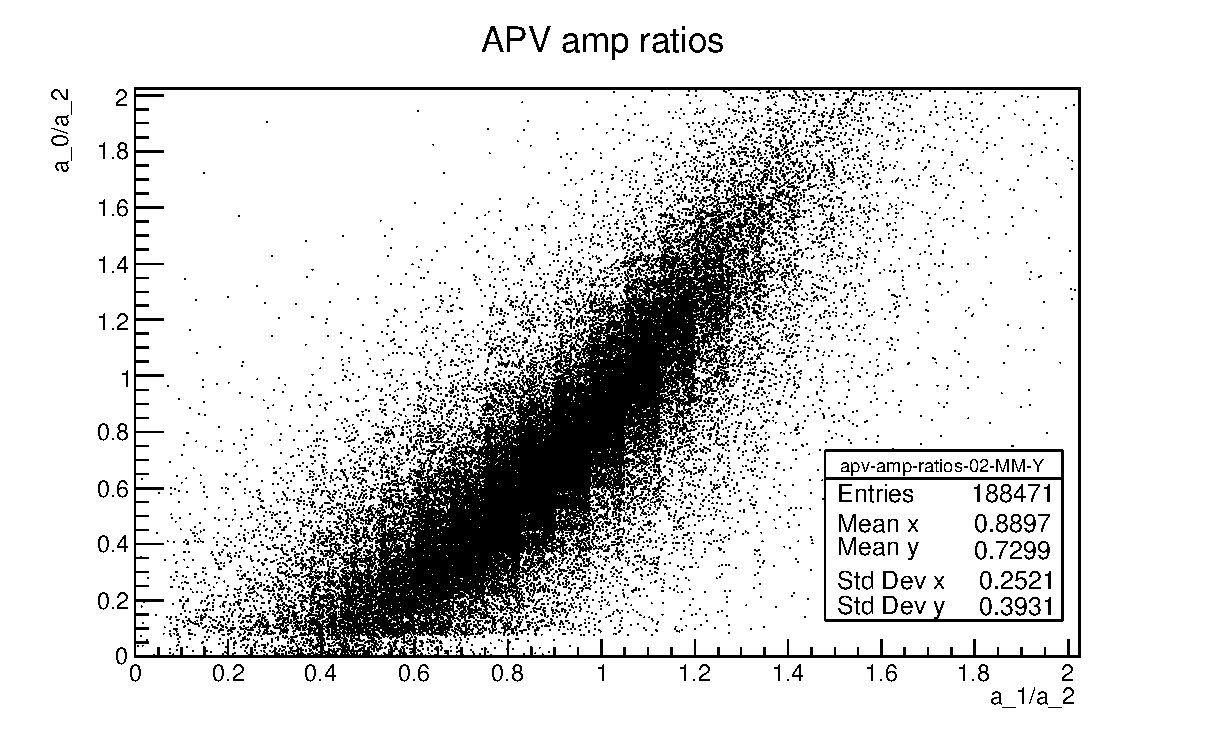
\includegraphics[width=0.45\linewidth]{images/illustrative/banana-example.eps}
    \caption{Пример распределения отношения амплитуд $r_{02}$ и $r_{12}$ переднего
    фронта сигнала микроструктурного детектора}
    \label{fig:banana-histogram}
\end{figure}

\subsection{Реконструкция измерений от тонкостенных трубок}

%Станции тонкостенных газоразрядных трубок предоставляют информацию
%о времени развития электронной лавины $t'$ в рабочем объёме конкретной
%трубки относительно времени срабатывания триггера. В $t'$ включено
%время пролёта частицы до трубки $\delta t$, которое для большинства
%релятивистских частиц (мюонов и электронов) принимается постоянным.
%Так, например, времяпролётная разница на дистанции в десять метров
%для электронов в $1~\text{ГэВ}$ и $100~\text{ГэВ}$ составляет
%менее $1~\text{пс}$, для мюонов -- менее $200~\text{пс}$, в то время
%как характерное время дрейфа лавины в трубке обычно составляет десятки
%наносекунд -- $20~\text{нс}$ для трубок диаметром $2~\text{мм}$
%и $50~\text{нс}$ для трубок $6~\text{мм}$. При принципиально-достижимом
%координатном разрешении в детекторах такого типа в $200~\text{мкм}$
%эта разница во временах для лептонов высоких энергий несущественна.
Станции тонкостенных газоразрядных трубок регистрируют время развития
электронной лавины $t'$ в рабочем объёме каждой трубки относительно
сигнала триггера. В это время включено также запаздывание
частицы $\delta t$, которое для большинства релятивистских частиц
практически постоянно. Так, например, различие
во времени пролёта на расстоянии десяти метров между электронами с
энергией $1~\text{ГэВ}$ и $100~\text{ГэВ}$ составляет менее $1~\text{пс}$,
а для мюонов~-- менее $200~\text{пс}$, тогда как характерное время
дрейфа лавины в трубке находится на уровне десятков наносекунд:
около $20~\text{нс}$ для трубок диаметром $2~\text{мм}$ и порядка
$50~\text{нс}$ для трубок диаметром $6~\text{мм}$. При достижимом
координатном разрешении таких детекторов порядка $200~\text{мкм}$
указанные различия во времени пролёта для лептонов высоких энергий
не имеют существенного значения.

%По этой причине $t'$ определяется главным образом временем $T$ дрейфа
%электронной лавины в разрядном промежутке трубки от ближайшей точки
%ионизации до катодной проволоки с расстоянием $R$, которое в свою очередь
%в наибольшей степени зависит от давления и плотности газовой смеси.
Таким образом, величина $t'$ определяется главным образом временем $T$
дрейфа электронов в разрядном промежутке трубки от ближайшей точки
ионизации до катодной проволоки.

%Таким образом зависимость $R(T)$, хотя и имеет нелинейный характер,
%хорошо поддаётся аппроксимации различными аналитическими моделями.
%Параметры такой модели и составляют необходимую калибровочную
%информацию применяемую при определении радиуса
%изохроной цилиндрической поверхности задаваемой временем срабатывания~$T$.
Функция $R(T)$ имеет нелинейный характер, однако хорошо аппроксимируется
различными аналитическими моделями. Параметры такой аппроксимации и
составляют необходимую калибровочную информацию, используемую при
определении радиуса изохронной цилиндрической поверхности, соответствующей
данному времени срабатывания~$T$.

На рисунке~\ref{fig:straws-rt} изображена гистограмма полученная для
трубки диаметром $6~\text{мм}$, находящейся
позади адронного калориметра с наложенными поверх гистограмм аппроксимациями
зависимости $R(T)$.
%\begin{figure}[ht]
%    \centering
%    \includegraphics[width=0.95\linewidth]{images/illustrative/ST-RT.jpg}
%    \caption{Распределение $R(T)$ для нескольких трубок станции ST
%    диаметром $6~\text{мм}$ (ось времени инверирована)}
%    \label{fig:straws-rt}
%\end{figure}
\begin{figure}
    \centering
    \includegraphics[width=0.33\linewidth]{images//illustrative/ST-RT-single-mono.png}
    \caption{Распределение $R(T)$ для нескольких трубок станции ST
    диаметром $6~\text{мм}$, $R$ в мм, время в относительных единицах, ось времени инверирована}
    \label{fig:straws-rt}
\end{figure}
Большое количество срабатываний отстоящих от основной линии обусловлено
высоким фоном от вторичных частиц.

%Хотя определение радиуса изохронной поверхности таким образом представляет
%собой простую задачу (реализуемую при помощи единственного обработчика,
%применяющего калибровочные данные), последующее использование этой
%информации в
%алгоритмах трекинга требует привлечения нетривиальных
%алгоритмов либо на этапе предварительного поиска треков, либо
%в процессе подгонки параметров модели трека. В простейшем случае, проводят
%плоскость через оси трубок в одной координатной проекции, и отмечают
%линии пересечения изохронной поверхности с этой плоскостью. Получившиеся
%линии таким образом являются геометрическим местом возможного пересечения
%траектории частицы с плоскостью детектора с фиксированным разрешением.
%Поскольку для одной трубки таких линий образуется две, одной трубки
%недостаточно для определения координат частиц в одной проекции.
Хотя определение радиуса изохронной поверхности в таком подходе
представляет собой относительно простую задачу (реализуемую с помощью
единственного обработчика, использующего калибровочные данные),
дальнейшее применение этой информации в алгоритмах трекинга требует
привлечения более сложных методов -- как на этапе предварительного
поиска треков, так и при подгонке параметров модели трека. 

В простейшем случае через оси трубок в одной координатной проекции
проводится плоскость, и фиксируются линии пересечения изохронной
поверхности с этой плоскостью. Эти линии образуют геометрическое
место возможных точек пересечения траектории частицы с плоскостью
детектора при данном временном разрешении. Поскольку для одной трубки
возникают две такие линии, её информации недостаточно для определения
координаты частицы в одной проекции. Тем не менее, рассматривая показания
трековых детекторов в совокупности зачастую удаётся разрешить
возникающие неоднозначности. На рисунке~\ref{fig:evdisplay-new}
показана проекция пространственных примитивов изображающих
чувствительные объёмы детекторов MicroMega и станции трубок
совместно с допустимыми пределами разрешений (изображены
шириной $5\sigma$).

\begin{figure}[ht]
    \centering
    \includegraphics[width=0.5\linewidth]{images//illustrative/ST-evdisp-mono.png}
    \caption{Реконструкция треков по показаниям MicroMega (повёрнуты на $45^{\circ}$)
    со станициями тонкостенных разрядных трубок с изображением
    координатных разрешений и гипотезы трека с ковариационными конусами}
    \label{fig:evdisplay-new}
\end{figure}

%\begin{figure}
%    \centering
%    \includegraphics[width=0.5\linewidth]{images/illustrative/ST-evdisp.jpg}
%    \caption{Реконструкция треков в SPA}
%    \label{fig:evdisplay-new}
%\end{figure}

Возможны и более сложные алгоритмы реконструкции, учитывающие
трёхмерную структуру изохронных поверхностей в рамках одной станции
тонкостенных трубок~\cite{straws-peshekhonov2015}.

\subsection{Поиск треков}

%Задача предварительного поиска треков (англ. \emph{pattern recognition})
%состоит в выборе таких комбинаций пространственных объектов соответствующих
%отдельным измерениям, которые с заданной
%степенью правдоподобия могут образовывать трек частицы.
Задача предварительного поиска треков (англ. \emph{pattern recognition})
заключается в отборе таких комбинаций пространственных объектов,
соответствующих отдельным измерениям детектора, которые с заданной
степенью правдоподобия могут образовывать трек частицы.

%Среди множества существующих на сегодняшний день алгоритмов предварительного
%поиска треков~\cite{MankelTracking}, интерес представляет алгоритм
%CATS~\cite{catsc-JINR, catsc-discrete, catsc-nim, catsc-disto},
%(англ. \emph{cellular automata track search} -- в разное время авторы
%публиковали его формализацию в терминах <<эластичных>> нейронных сетей,
%и клеточных автоматов), который допускает весьма общую
%формулировку в силу независимости по отношению к конкретным
%геометрическим свойствам входных данных.
Среди многочисленных алгоритмов предварительного поиска~\cite{MankelTracking}
интерес представляет метод CATS
(англ. \emph{cellular automata track search})~\cite{catsc-JINR, catsc-discrete, catsc-nim, catsc-disto}.
В различных публикациях он излагался как в терминах <<эластичных>>
нейронных сетей, так и в формализме клеточных автоматов. 
Алгоритм допускает весьма общую формулировку в силу независимости по
отношению к конкретным геометрическим свойствам входных данных.

Формально задача, решаемая алгоритмом, может быть представлена следующим образом.
Пусть имеется
набор объектов $h_1,h_2, ...h_n$. Требуется найти такие
последовательности $(h_i,h_j,...h_m)$, для которых любая тройка
элементов $(h_{i-1},h_{i},h_{i+1})$ удовлетворяет заданному
условию $F(h_{i-1},h_{i},h_{i+1})=1$.
Основная идея состоит в эффективной стратегии обхода
объектов, позволяющей в большинстве случаев избежать прямого перебора
всех возможных комбинаций. Для этого алгоритм опирается на топологическую информацию
о <<слоях>> связанных с каждым объектом $h_i$. Каждому объекту сопоставляется
внутреннее состояние, обновляемых за конечно число итераций согласно
определённому правилу.

Пример работы алгоритма приведен на рисунке~\ref{fig:catsc-nim},
где приведены начальное и конечное состояния графа для синтетического набора
данных. Слои отмечены пунктирными
линиями, объекты $h$ (hits) изображены кругами, рёбра между парами
объектов -- сплошными линиями, а увеличенная толщина линии указывает
на больший вес соответствующей пары.

\begin{figure}
    \centering
    \includegraphics[width=0.45\linewidth]{images//illustrative/catsc-quote-it1.png}
    \includegraphics[width=0.45\linewidth]{images//illustrative/catsc-quote-it6.png}
    \caption{Начальное и конечное состояние графа связности после шести итераций алгоритма CATS~\cite{catsc-nim}}
    \label{fig:catsc-nim}
\end{figure}

В простейшем случае, в качестве объектов $h$ выбираются пространственные
точки, а условием $F$ является условие на максимальный пространственный
между ними $F(h_{i-1},h_{i},h_{i+1}): \angle(h_{i-1}h_i) (h_i h_{i+1}) < \theta_{th}$.

В результате время работы алгоритма оказывается существенно ниже
прямого перебора, в худшем случае ($\theta_{th} =\pi$) имея
сложность $\mathcal{O}(Ln^3)$, где $L$ -- число слоёв,
и $n$ -- число объектов $h$. Практически, сложность регулируется
функцией-фильтром, и при трудоёмкости фильтра~$\mathcal{O}(1)$ алгоритм
имеет сложность $\mathcal{O}(Ln^2)$. Наивный перебор троек $h$
с фильтрующей функцией дающей в среднем $d$ объектов в следующем слое
имеет сложность $\mathcal{O}(n^3 d^{L-3})$. Без фильтрующей функции
максимальная сложность возрастает экспоненциально $\mathcal{O}(n^L)$,
однако главное преимущество CATS перед наивной реализацией состоит
в устранении экспоненциального роста памяти, необходимой для хранения
гипотез. Алгоритм сводит задачу к итеративному линейному обходу
двунаправленного графа.

В оригинальных работах~\cite{catsc-JINR, catsc-discrete, catsc-nim, catsc-disto}
$h_i$ рассматриваются как пространственные точки $h_i:=\vec{r}_i$, или кортежи из
координат и времени $h_i:=(\vec{r}_i,t_i)$, в то время как алгоритм сам по себе
не подразумевает какого-то конкретного набора свойств, а требует
только того, чтобы определена функция $F:h_{1,2,3} \rightarrow \{0,1\}$.

Дополнением оригинального алгоритма является определение весовых
коэффициентов возвращаемых функцией-фильтром, то есть в более общем
случае $F: F(h_{1,2,3}) =w_j, ~w_j \in \mathbb{R_1}$. Кроме того, после
конструирования графа связности стратегия извлечения гипотез (обхода точек)
может допускать различные формы, что в оригинальных работах не
рассматривается. В частности, в случае когда одна и более гипотез $T_p, T_q$
претендуют на один и тот же сегмент $T_p \cap T_q = (h_i, h_j)$ выбор в пользу
той или иной гипотезы целесообразно бывает разрешать руководствуясь различными
критериями. Стратегии обхода результирующего графа реализованы в виде
программных модулей.

\subsection{Аппроксимация треков}

Классическая задача восстановления трека по измеренным
координатам в NA64 решалась различными методами.
Наиболее недавним является применение фильтра Калмана~\cite{kalman-1960},
реализованного библиотекой GenFit2~\cite{Genfit2_Rauch_2015}
в различных редакциях и с дополнениями оригинального алгоритма, из которых
наибольший практический интерес в контексте NA64
представляют
DAF (англ. \emph{deterministing annealing filter}~\cite{daf-track-fitting})
и KRF
(англ. \emph{Kalman filter with reference track}~\cite{krf-kalman-w-reference-track}).

Для подгонки параметров модели треков в условиях сложной геометрии
применяется KRF.
Его особенность по сравнению с оригинальным алгоритмом фильтра Калмана
состоит в том, что линеаризация уравнений переноса и измерений
выполняется не в малой окрестности предсказания, а
относительно заранее заданной опорной траектории,
обновляемой затем в несколько итераций. Этот приём позволяет снизить
систематические искажения при аппроксимации трека в
неоднородном магнитном поле, с учётом эффектов множественного
рассеяния (например, при проведении трека через калориметр).
Использование данного метода оправданно в сочетании с алгоритмами
поиска треков, которые задают разумное начальное приближение
для опорной траектории -- таких, как CATS~\cite{catsc-nim}.

DAF решает иную задачу: выбор согласованного подмножества
измерений в условиях неоднозначностей и загрязнений. В
его основе лежит назначение весов отдельным хитам с
последующей процедурой итеративного обновления весов. Вначале все
измерения вносят вклад в $\chi^2$-функцию, затем веса асимптотически
сходятся к согласованной гипотезе. В пределе это приводит к отбору
хитов, принадлежащих правдоподобной гипотезе с эффективным
исключением ложных срабатываний.


\section{Предметно-ориентированные языки}

Для решения локальных задач возникающих в узкой предметной области,
часто прибегают к конструированию т.н. предметно-ориентированных
формальных языков~(англ. \emph{domain-specific languages}, также
<<проблемно-ориентированные языки
программирования>>, \acrshort{dsl})~\cite{DSL-Fowler2011}. Такие искусственные
языки не обязательно обладают качествами присущими языкам программирования
общего назначения: они могут не обладать полнотой по Тьюрингу (язык
запросов SQL в редакции 1992 года~\cite{ISO90751992}, язык
регулярных выражений~\cite{thompson1968programming},
не иметь выразительных средств для арифметических операций или операций со
строками, абстракциями ввода-вывода и т.п. Взамен такие языки
предоставляют специализированные выразительные средства для решения узкого
класса прикладных задач посредством более компактных нотаций.

В качестве примеров таких языков в \acrshort{hep} можно привести
математическую нотацию численных функций и логических предикатов
<<TFormula>> программного окружения ROOT \cite{ROOT-framework} или язык численных
функций встраиваемый в интерпретатор GDML в~\cite{Berra2011Geant4SO}.

Создание программных инструментов для интерпретации \acrshort{dsl}
возможно при помощи автоматизированных средств, на основе
формализованной специальным образом грамматики~\cite{alfred2007compilers}.
Средства вводят следующие ограничения на уровнях лексического
разбора~(англ. \emph{lexer}) и семантического анализатора~(англ. \emph{parser}):
\begin{itemize}
    \item Лексический интерпретатор поддерживает регулярные
    грамматики (тип 3 по иерархии Хомского~\cite{chomsky1956three}),
    т.е. эквивалентные детерминированному конечному автомату. Такие грамматики
    позволяют право- или леворекуррентные определения правил, однако
    не их сочетания.
    \item Парсер поддерживает более узкий набор грамматик  LALR(1)
    (\emph{look-ahead, left-to-right}, тип 2 по иерархии Хомского) ---
    анализатор с ограниченным односимвольным упреждением на основе
    левостороннего восходящего разбора.
\end{itemize}
Эти ограничения позволяют конструировать довольно сложные
грамматики, вполне достаточные для реализации небольших \acrshort{dsl},
не требующих полной выразительной мощности контекстно-свободных
грамматик и не содержащих конструкций с неоднозначным синтаксисом
или контекстно-зависимыми правилами.
%, что актуально в языках программирования общего назначения.

Формальные описания грамматик языков и программ реализующих
примитивы исполнения вынесены в приложение~\ref{appendix:dsl-grammars}.

\subsection{Числовой идентификатор детектора и язык селекторов}

Одним из частых предусматриваемых обобщающих сценариев использования
конвейерного шаблона проектирования является применение отдельного
обработчика к выборке объектов по ключу (идентификатору детектора)
в коллекции объектов. Например, в задачах анализа и
онлайн-диагностики детектора
нужно построить гистограмму величины ассоциированной с конкретным
детектором. В другом случае -- назначить различные обработчики
разным группам детекторов. В этих случаях целесообразно предусмотреть гибкий
механизм определения подмножества посредством специализрованных
выражений.

В подобных случаях нередко прибегают к индексированию детекторов и связанных
с ними данных посредством строковых идентификаторов. Так например, в системе
сбора данных COMPASS и NA64 внутренняя номенклатура идентификаторов детекторов
построена в соответствии с грамматикой описывающей имя детектора
в форме слова <<имя>> + <<номер станции>> (см. подробнее в приложении~\ref{appendix:dsl-grammars}).

Тогда выборку детекторов можно произвести на основе
какого-нибудь \acrshort{dsl} предназначенного для поиска строкового
соответствия~--- например языка регулярных выражений или
языка поисковых шаблонов Unix~(англ. \emph{wildcard}~\cite{wildcards-mcilroy1987research}).

На практике, эта грамматика в эксперименте COMPASS носит лишь
рекомендательный характер. Сложные станции этого спектрометра, состоящие из
нескольких координатно-чувствительных плоскостей (зон, в поперечном
сечении) обуславливают необходимость дополнительного подразделения. Так, по мере
развития эксперимента COMPASS в номенклатуру его детекторов
оказались введены такие элементы как \texttt{ST03ub}, \texttt{MA01c},
\texttt{MP03MX1}, вовсе не следующие формальным правилам общим более чем
для единственной станции. Выбор станции или плоскости всё ещё можно
реализовать при помощи строковых \acrshort{dsl} -- то есть, с одной стороны это
довольно гибкий подход.

С другой стороны отсутствие формальной грамматики, во-первых
приводит к неоднозначности при выборе отдельных чувствительных элементов,
затрудняет выбор связанных с ними транзитивно (в рамках модели
события) экземпляров данных.
% нужны ли тут примеры? что если я хочу выбрать только стриповые части
% микромег без пиксельных частей?
Во-вторых, операции строкового сравнения в общем случае менее
эффективны, чем сравнение числовых идентификаторов. С учётом того,
насколько часты на практике такие запросы к объектной
модели (поиск по ключу, различные условия выборки и фильтрации),
целесообразно предусмотреть программное средство для биективного
преобразования строковых и числовых идентификаторов для перечисления
номенклатуры детекторов. При этом всё ещё возможно предусмотреть
определённую свободу в именовании, часто диктуемую ситуативным
удобством при размещении детекторов на пучке и подключении
электроники.

Большим преимуществом числовых идентификаторов является удобство
их использования в ассоциативных контейнерах на основе бинарных
деревьев поиска (в частности, красно-чёрных деревьях реализованных
в библиотеке шаблонов STL C++). Это позволяет существенно упростить
работу с объектной моделью события в C++, снабдить порядок
итерирования дополнительной семантикой, обеспечить эффективный
компромисс между быстродействием при прямых запросах по ключу
и использованием памяти. Обращения к такому контейнеру не подразумевают
вычисления хеш-сумм, символьных сравнений и др. Поиск по ключу имеет
сложность $O(\text{log}~n)$.

%В дальнейшем, в рамках работы будем ссылаться на язык и его реализацию
%его интерпретатора по имени
%<<DSuL>> (\emph{detector selection micro-language}).

\subsection{Язык запросов модели события}

Объектная модель события снабжённая рефлексией сама по себе
уже позволяет строить обобщённые обработчики в рамках конвейерного
шаблона проектирования.

Так, например, достаточно определить класс обработчика строящего
одномерную гистограмму случайной величины, параметризуемый
идентификатором ссылающимся на определённый числовой атрибут события,
чтобы реализовать возможность построения всех одномерных гистограмм
любого атрибута в событии. Таким образом, введение новых атрибутов
посредством выведения шаблонов не требует никаких дополнительных
операций со стороны разработчика для создания гистограмм вводимых новым
типом значений.

В качестве идентификатора атрибута можно использовать нотацию близкую
к принятой в C++: например, выражения \texttt{SADCHits.time} или
\texttt{APVClusters.hits.x} достаточно близки к нотации разыменования
атрибутов в C++.
%Тем не менее, такая запись во втором случае допускает
%различие в интерпретации -- неясно, какая из двух коллекций (\texttt{APVClusters}
%или \texttt{APVClusters.hits}) должна итерироваться первой.

Помимо этого, нередки случаи, когда необходимо выполнить некоторые (элементарные)
преобразования с полями события, или применить фильтрацию на уровне
атрибута с типом-коллекцией. % так, как это определено, например, в DSuL.

С этой целью в программном окружении предусмотрена интеграция с
\acrshort{dsl} предназначенным для работы с потоками организованных
иерархически
объектов с заранее известной схемой (топологией). Он поддерживает базовые
операции фильтрации и арифметики значений, однако не позволяет изменять
топологию данных (что является одним из сознательных ограничений по сравнению с
более универсальными \acrshort{dsl}, такими как SQL или GraphQL \cite{graphql-comparative}).

Основными вариантами использования языка являются:
\begin{itemize}
    \item Задание логических условий для дискриминации событий или элементов
    коллекций внутри события (таких, как кластеры или треки).
    \item Задание генераторных выражений для построения N-мерных гистограмм.
    \item Задание генераторных выражений для представления данных физических
    событий в табличном виде.
\end{itemize}
Во всех случаях, язык должен допускать арифметические вычисления,
определение новых элементов объектной модели (существующих в рамках
запроса), применение агрегатных функций над выборками.

\subsection{Описание калибровочных данных}

%В экспериментальной физике нередко возникает необходимость представления
%информации с хронологической привязкой к астрономическому времени, либо
%в соответствии с внутренней хронологической номенклатурой (например, к
%периодам набора статистики, когда конфигурация установки в достаточной степени
%неизменной). Источником таких данных могут быть как внешние измерения:
%результаты геодезической съёмки, обеспечивающие относительную геометрическую
%привязку детекторов, сведения о температуре, влажности и давлении в
%экспериментальном зале, значения токов газовых смесей в рабочих объёмах
%установки и т.д. К тому же классу относятся и данные, регистрируемые
%непосредственно подсистемами детекторов: коэффициенты масштабных
%преобразований (амплитудных и временных), пороговые значения для
%подавления фона и шумов, а также коэффициенты, определяющие шкалы
%преобразований для различных типов аналого-цифровых и цифровых
%преобразователей. В дальнейшем под калибровочной информацией будем
%понимать весь объём данных, не относящихся непосредственно к
%экспериментальной статистике, но требующих временной привязки и
%используемых в алгоритмах обработки и реконструкции.
%
%В общем случае задача управления таким набором данных, подразумевающая
%прежде всего быструю операцию поиска по хронологическому ключу, и, с
%меньшим приоритетом, -- операции вставки и удаления записей, решается при
%помощи реляционных таблиц организованных под управлением различных СУБД.
%
%При этом задача интеграции СУБД с программами обработки, в особенности
%на ранних этапах разработки и прототипирования, нередко представляет
%определённую техническую сложность из-за необходимости сопровождения
%участков программы отвечающих за преобразование табличных данных в массивы
%записей (экземпляры объектной модели), разрешение коллизий, сопряжение
%информации из различных таблиц.
%
%С целью упростить процедуру ранней разработки и предоставить инструмент
%облегчающий дальнейший перенос калибровочной информации под управление
%СУБД, было разработано программное решение опирающееся на представление
%калибровочной информации в виде текстовых таблиц.
В общем, под \emph{калибровочной информацией} в данной работе понимается
совокупность данных, не относящихся непосредственно к событиям, но
требующих временной привязки и необходимых для алгоритмов обработки и
реконструкции. К такому классу относятся, например, результаты геодезических
измерений, обеспечивающие относительное позиционирование детекторов,
сведения о внешних условиях (температура, влажность, давление, параметры
газовых смесей), а также коэффициенты и пороговые значения, определяемые
по показаниям самих детекторов и задающие масштабные шкалы
измерительных каналов.

На уровне отдельных обработчиков работа с калибровочной информацией
ограничена задачей быстрого поиска по временным ключам.
Традиционно такая задача решается с
использованием реляционных таблиц под управлением \acrshort{dbms}.
Однако на стадии прототипирования интеграция с \acrshort{dbms}
может быть затруднена необходимостью преобразования табличных структур в объекты,
согласования информации из разных таблиц и обработки коллизий.

С целью упростить эти процедуры на ранних этапах разработки и
обеспечить возможность последующего переноса данных в полноценные
\acrshort{dbms} было реализовано программное решение, основанное на
представлении калибровочной информации в виде текстовых таблиц.
%Программное решение представлено библиотекой шаблонных процедур,
%работающих с индексом временных интервалов которым в соответствие
%поставлены записи состоящие из идентификатора артефакта и типа
%данных.
Решение предоставляется в виде библиотеки шаблонных
процедур, работающих с индексом временных интервалов. Интервалам
в индексе сопоставляются записи, включающие идентификатор
артефакта-источника и соответствующий тип данных.

%Индекс представляет собой шаблонный класс
%параметризуемый произвольным типом ключа для которого посредством
%шаблонной специализации C++ задаются операция сравнения и нулевой
%элемент соответствующий открытому интервалу.
Индекс построен как шаблонный класс, параметризуемый произвольным
типом ключа. Для этого ключа посредством специализации шаблонного
класса C++ задаётся единственная операции сравнения, а также определяется
нулевой элемент, интерпретируемый как открытый интервал.

Библиотека предоставляет реализации процедур для рекурсивного
разбора текстовых файлов с табличной информацией и преобразования
её в пользовательские типы данных (посредством шаблонной
специализации). Подразумевается, что документы помимо таблиц могут
содержать разметку (метаданные) влияющую на
лексическое преобразование. Так важным практическим вариантом
использования  является переопределение отдельных элементов для
временных подинтервалов, определение неполных данных, фрагментация
таблиц с целью более гибкой настройки логики применения данных,
поддержка арифметических преобразований (встроенный интерпретатор
формул) и т.д.
Библиотека содержит средства для рекурсивного разбора текстовых файлов
с табличными данными и их преобразования в пользовательские типы
(через механизмы статического полиморфизма). Предполагается,
что документы могут включать не только таблицы, но и метаданные,
аннотирующие калибровочную информацию и влияющие на процесс
лексического анализа. На практике это позволяет реализовывать
такие сценарии, как переопределение отдельных элементов для
временных подинтервалов, задание неполных данных, фрагментация
таблиц.

Лексический разбор документов организован на основе регулярных
выражений с настраиваемой грамматикой, которая описывает
искусственный язык разметки, подобный
языку описания гипертекстовых документов HTML~\cite{berners1989information},
языку спецификации каскадных стилевых таблиц CSS~\cite{lie1996cascading}),
или языку конфигурационных файлов YAML~\cite{yaml-rfc9512}.
Лексический разбор также включает интерпретатор
арифметических выражений для выполнения арифметических
преобразований (делегируется \texttt{TFormula}~\cite{ROOT-framework}).
Пользовательский код
может изменять разделители табличной разметки, способы
интерпретации и маркеры метаданных, учитывать информацию
о путях размещения артефактов.

Решение оптимизировано под цикл разработки подразумевающий
управление калибровочными размещёнными в файлах или иных артефактах
с иерархической моделью доступа, с последующей синхронизацией
сетевым сервисом настроенным на автоматическое
отслеживание ресурса на котором публикуются документы.

%В заключении нужно отметить, что хотя преобразование таблиц на этапе
%индексации артефактов не выполняется (таблицы интерпретируются только при запросе
%по ключу), необходимость построения индекса является
%естественным ограничением такой архитектуры.
Следует отметить, что преобразование таблиц в процессе индексации
не выполняется: они интерпретируются лишь при обращении по ключу.
Это обеспечивает заявленную сценарную гибкость, однако сама необходимость
построения индекса выступает архитектурным ограничением предложенного
подхода.
\section{Форматы данных}

Объектная модель события представляет данные в программе,
в то время как задачу хранения данных нужно решать с
привлечением различных стандартизированных средств.

Коротко рассмотрим реализации кодировщиков моделей события
и выходных данных.

\subsection{Форматы хранения событий}

Использование различных форматов хранения данных в программном окружении
является одним из основных предметов модульной архитектуры.
Благодаря средствам статического полиморфизма поддержка
различных форматов выполняется в виде шаблонных
специализаций, основанных на шаблонном обходе топологии типов.

Для представления данных о событии применялись следующие форматы:
\begin{itemize}
    \item ROOT \texttt{TTree}, как основной формат принятый
    в экспериментальной физике высоких энергий,
    \item Apache Avro~\cite{avro-spec}, компактный и быстрый
    формат обмена иерархическими
    данными со статической типизацией.
\end{itemize}

Также применялись форматы HDF5~\cite{hdf5-std},
и Google Protocol Buffers~\cite{protobuf-spec}. Хотя их использование
в NA64 прекратилось, для указания на универсальность подхода следует отметить,
что интеграция с ними
осуществлялась в той же парадигме автоматического выведения
реализации на основе статического полиморфизма.

На рисунке~\ref{fig:data-sources-example} приведена диаграмма
классов содержащая пример модульной системы на основе
абстрактных классов \texttt{AbstractDataSource} и
\texttt{AbstractEventHandler}.
%Компоненты интегрирующие
%Apache Avro или предоставляющие источник данных COMPASS DAQ
%могут отсутствовать в системе

\begin{figure}
    \centering
    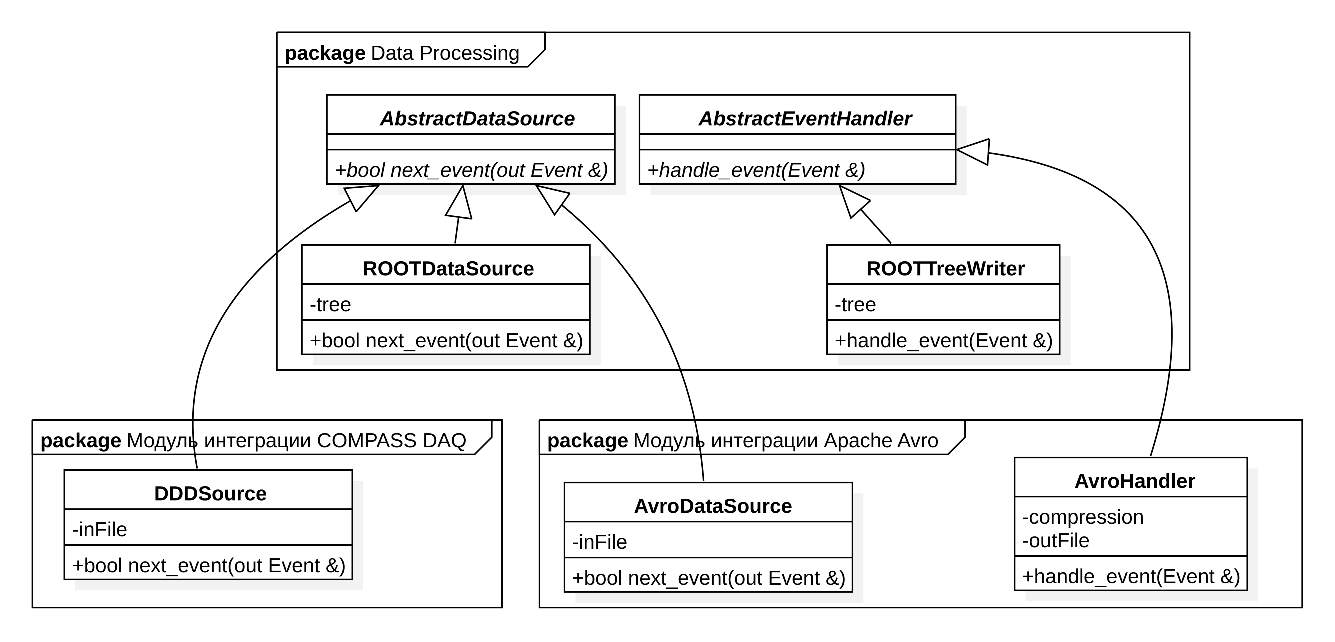
\includegraphics[width=0.95\linewidth]{images/illustrative/data-sources-example.eps}
    \caption{Диаграмма классов иллюстрирующая отношения классов реализующих различные форматы хранения событий}
    \label{fig:data-sources-example}
\end{figure}

Как и в случае с объектной моделью события, рассмотренной ранее,
автоматическая генерация декодировщиков данных относится преимущественно
к внутренним протоколам программного окружения. Интеграция с внешними
источниками осуществляется через отдельные модули,
требующими участия разработчика для сопровождения.

Так, в частности, важнейшим источником является декодирование данных,
считанных напрямую из системы сбора данных (DAQ), которое опирается
на библиотеку кодирования COMPASS~\cite{compass-daq}.

Таким образом, модуль реализующий интерфейс источника данных обычно
является промежуточным слоем между библиотекой и ядром системы.

\subsection{Иерархия детекторов в выходных данных}

Класс \texttt{TDirAdapter} (из окружения ROOT) предоставляет
часто используемые операционные примитивы при отображении
множества детекторов в связанный
набор экземпляров подкласса \texttt{TObject} допускающих
хранение внутри \texttt{TDirectory}. В таком виде удобно
размещать большие наборы гистограмм и
графиков соответствующих индивидуальным детекторам в рамках одного
обработчика. Так, например, с применением идентификаторов детектора,
наглядную иерархию объектов отвечающую
логической структуре детектора изображённую на
рисунке~\ref{fig:tobject-hierarchy} можно получить подстановкой
семантических элементов идентификатора в простой текстовый шаблон.

\begin{figure}
    \centering
    \includegraphics[width=0.25\linewidth]{images//illustrative/items-structure-in-root-file.png}
    \caption{Иерархия объектов внутри \texttt{TFile} порождаемая
    идентификатором детектора на основе шаблонных путей}
    \label{fig:tobject-hierarchy}
\end{figure}

Обработчики включающие \texttt{TDirAdapter} обычно
предусматривают переопределение шаблонов путей для адаптации к
конкретным пользовательским приложениям в тех случаях когда
спецификация входного файла каким-то образом ограничена.

\subsection{Извлечение характеристик распределений}

Например, часто возникающая практическая задача отыскания
коэффициентов распределений на основе особенностей различных
спектров может быть обусловлена в виде короткого конфигурационного
файла задающего:
\begin{itemize}
    \item Шаблон имени гистограммы при помощи регулярных
    выражений с именованными группами захвата для извлечения
    имени детектора и индекса элемента,
    \item Обозначения особенности на
    спектре -- например <<первый минимум по порядку>>,
    <<второй максимум по высоте>>.
\end{itemize}

\begin{figure}
    \centering
    \includegraphics[width=0.5\linewidth]{images//illustrative/tmt-fit-example.png}
    \caption{Пример автоматического выделения основного пика во временном
    распределении мюонного сигнала в вето-детекторе}
    \label{fig:placeholder}
\end{figure}

Обобщение практики применения таких процедур показывает, что количество
особенностей сравнительно невелико, и в большинстве случаев логика,
необходимая для калибровки или автоматизированного анализа, может быть
задана в виде компактной спецификации.

\section{Калибровка детекторов}

\subsection{Калибровка детекторов просматриваемых фотоумножителями}

В предположении, что в отдельном чувствительно объёме детектора
просматриваемом \acrshort{pmt} зависимость уровня сигнала $A$ от
выделившейся в рабочем объёме детектора энергии~$E$ с хорошей
точностью аппроксимируется линейной
зависимостью~$E \simeq C \cdot A$,
калибровка соответствующего детектора состоит в отыскании
коэффициентов~$C$ для известной энергии $E$ и измеренной амплитуды
сигнала~$A$.

Эти коэффициенты трудно или невозможно посчитать заранее, поскольку
они зависят от множества технических и физических условий стационарных
лишь в некотором приближении, включающих уровень высокого напряжения
питающей системы, параметры входных и выходных каскадов элементной
базы, напряжения на динодах \acrshort{pmt}, качества оптического контакта
и т.д.
%~\acrshort{pmt} на динодной системе, а этот уровень в свою очередь выбирается таким
%образом, чтобы обеспечить достаточное энергетическое
%разрешение \acrshort{pmt} в счётном режиме работы -- обычно так,
%чтобы номинальная энергия пучка не превышала верхнюю
%границу~\acrshort{adc}. При этом, коэффициент $C$ подвержен дрейфу
%вследствие различных физических процессов в выходном каскаде
%питающей аппаратуры, в динодной системе и на фотокатоде,
%в веществе детектора.
В силу случайного характера этих процессов
обусловленных в основном индивидуальными параметрами детектора
и \acrshort{pmt}, отыскание калибровочных коэффициентов $C$
можно осуществить на основе процессов с известным спектром.
Таким эталоном могут служить, например, мюоны, для которых обычно
хорошо известен пик минимально ионизирующих частиц~(\acrshort{mip}),
атмосферные мюоны, или моноэнергетические пучки искусственного
происхождения, для которых можно получить спектральные
оценки из моделирования методами Монте-Карло.




%\section{Визуализация событий}

\begin{figure}
    \centering
    \includegraphics[width=0.5\linewidth]{images//illustrative/ecal-evidplay-example-3d.png}
    \caption{Визуализация события в ECAL}
    \label{fig:event-display-ecal-only}
\end{figure}

\begin{figure}
    \centering
    \includegraphics[width=0.25\linewidth]{images//illustrative/event-display-mult.png}
    \caption{Общий вид приложения}
    \label{fig:event-display-3d}
\end{figure}


\section{Калибровка электромагнитного калориметра}

\subsection{Псевдообратная матрица}

В линейном приближении зависимость энерговыделения в $i,j$-ой ячейке $E_{ij}$
от зарегистрированной амплитуды выражается как $E_{ij} = C_{ij} A_{ij}$, где
$C_{ij}$ -- калибровочный коэффициент. Тогда то свойство центральных
ячеек $I_c = ((2,3), (3,3))$, что ECAL практически полностью поглощает
всю энергию первичной частицы $E_{beam}$ в случае попадания частицы в них
можно записать следующим образом:
\begin{equation}
    E_{beam} = \sum\limits_{i,j}^{5,6} C_{ij} A_{ij},
    \label{eq:ecal-eSum}
\end{equation}
то есть, для герметичного калориметра, сумма энергий выделившихся во всех
ячейках должна быть равна номинальной энергии пучка для случая попадания
частицы в центральную часть (ячейки $(2,2)$ или $(2,3)$). Выражение
\eqref{eq:ecal-eSum} задаёт систему линейных уравнений.

Для идеального детектора можно было бы рассматривать $A_{ij}$ в смысле
средних значений для $N$ событий~$\bar{A}_{ij}=\mathop{\mathbb{E}}\limits_{n \in N}[A_{ij} + \delta A_{n,ij}] \simeq A_{ij}$, и тогда задача калибровки свелась
бы к решению простой \acrshort{sle}. В реальности решения~\eqref{eq:ecal-eSum} для
каких-нибудь тридцати событий в общем
случае не существует, потому что для каждого события $n$
выражение~\eqref{eq:ecal-eSum} приобретает случайные добавки в каждой ячейке:
\begin{equation}
    E_{beam} + \delta E_n = \sum\limits_{i,j}^{5,6} \left( C_{ij} (A_{ij} + \delta A_{n,ij}) + \delta E_{n,ij} \right),
    \label{eq:ecal-eSum-deviating}
\end{equation}
где $\delta E_n,~\delta A_{n,ij}$ -- случайные значения отклонений энергии
частицы и зарегистрированной амплитуды, а $\delta E_{n,ij}$ -- физические флуктуации
в ячейке.

Тем не менее в предположении, что для заданной средней координаты
падения частицы в среднем, энерговыделение в ячейке имеет нормальный
закон распределения $E_{ij} \sim \mathcal{N}(\bar{E}_{i,j},\sigma_{E,ij})$,
выражение \eqref{eq:ecal-eSum} задаёт переобусловленную \acrshort{sle},
которую можно решить методом псевдообратной матрицы. Такая численная процедура
решает задачу минимизации среднего квадрата отклонения, и позволяет получить
приближённое решение~\eqref{eq:ecal-eSum}. Тем не менее большое значение
для периферийных ячеек имеют флуктуации энерговыделения~(то есть, такой алгоритм
в общем случае численно-неустойчив).
Это приводит к большой ошибке в определении калибровочных
коэффициентов, если рассматривать только центральные ячейки для которых
выполняется условие герметичности.

Алгебраическую постановку задачи можно расширить, если рассмотреть
интеграл функции энерговыделения в объёме ячейки $v_{ij}$:
\begin{equation}
    E_{ij} =\int\limits_{v_{ij}} \frac{dE_{cnv} (r)}{d r} dv, \quad E_{beam} = \sum\limits_{ij}^{5,6} E_{i,j},
\end{equation}
где средняя объёмная дифференциальная плотность
энерговыделения $d E_{cnv}(r)/dr$ выражается через интегральную свёртку
проекции пучка $P$ на переднюю грань калориметра и функции объёмного
профиля ливня~$d E_{EM}(r)/dr$:
\begin{equation}
    E_{cnv}(r) = P * E_{EM}
        = \int\limits_{V} P(\rho_x,\rho_y) \frac{dE_{EM} (r -\rho)}{d \rho} d\rho.
    \label{eq:cnv-em-shower}
\end{equation}

Нужно заметить, что выражение \eqref{eq:cnv-em-shower} пренебрегает угловой
зависимостью импульсов частиц. В более общей постановке $E_{cnv}$
зависит от угла попадания частицы в калориметр, а $d E_{EM}/dr$ должна
учитывать анизотропию развития ливня в сэмплирующем калориметре.

Таблица значений $E_{ij}$ определяется относительно центральной
ячейки $i=0,j=0$. Таким образом для калориметра $5\times6$
$i$ изменяется в диапазоне от $-5$ до $5$ и $j$ от $-6$ до $6$.

\subsection{Координатная неоднородность}

Неоднородность отклика установки по отношению к точке попадания
инициирующей частицы в ECAL
иллюстрирует рисунок \ref{fig:ecal-cell-nonhomo}. На рисунке~\ref{fig:ecal-abs-edep}
изображена двумерная гистограмма заполненная координатным распределением
точки попадания частицы в локальных координатах, полученная экстраполяцией
на основе данных трекера. Резкий внешний круговой контур
соответствует проекции чувствительного элемента пучкового счётчика.
Локальные изменения плотности пятна соответствуют
конструктивным элементам ячейки калориметра в торцевой проекции изображённой
на рисунке~\ref{fig:ecal-abs-error}~--- по сравнению с центральной частью ячейки заметны значительные (до $10~\text{ГэВ}$) ошибки в оценке энергии ливня
при попадания частицы в армирующие стальные стержни
и на границах ячейки.
%или в отверстия через
%которые через ячейку проходят светопроводящие волокна.

%\begin{figure}
%    \centering
%    \includegraphics[width=0.95\linewidth]{images//illustrative/ECAL-cell-beamspot-nonhomo.png}
%    \caption{Распределение координат первичных частиц на фронтальной
%    грани калориметра ECAL и фотография торцевой части ячейки}
%    \label{fig:ecal-cell-nonhomo}
%\end{figure}

\begin{figure}
    \centerfloat{
        \hfill
        \subcaptionbox{Среднее энерговыделение\label{fig:ecal-abs-edep}}{\includegraphics[width=0.47\linewidth]{images//illustrative/image.png}}
        \hfill
        \subcaptionbox{Абсолютная ошибка реконструкции\label{fig:ecal-abs-error}}{
            \includegraphics[width=0.47\linewidth]{images//illustrative/ecal-beam-error.png}}
    }
    \caption{Зависимость реконструированного среднего энерговыделения и ошибки от координат на передней грани ECAL}
    \label{fig:ecal-cell-nonhomo}
\end{figure}

Нестабильность поля отклоняющей магнитной системы способна вызывать
значительные горизонтальные колебания пучка. Рисунок~\ref{fig:counts-fluctuating}
иллюстрирует изменение числа зарегистрированных частиц из-за
кратковременного дрейфа координаты вызванного неполадками в питающей
системе отклоняющего магнита. В качестве наглядного примера на
рисунке~\ref{fig:edep-fluctuations} приведена
скоррелированная зависимость изменения энерговыделения в центральной ячейке.

\begin{figure}
    \centering
    \includegraphics[width=0.95\linewidth]{images/illustrative/run-10775-t2-s0pv0-s2pv1.pdf}
    \caption{Развёртка числа частиц зарегистрированных на мишени (T2) и
    числа отсчётов пучковых счётчиков по номеру спилла}
    \label{fig:counts-fluctuating}
\end{figure}

\begin{figure}
    \centering
    \includegraphics[width=1\linewidth]{images//illustrative/edep-fluctuations-run10775.png}
    \caption{Развёртка амплитудных показаний центральной ячейки ECAL}
    \label{fig:edep-fluctuations}
\end{figure}

Этот пример наглядно иллюстрирует причины загрубления энергетического
разрешения калориметра и необходимость привлечения информации о
треке частицы для оценок линейности калориметра, собственного
разрешения калориметра и т.д., поскольку ошибка энергетической
реконструкции вызванная неоднородной чувствительностью калориметра
может достигать нескольких процентов энерговыделения.

\subsection{Разрешение и линейность}

На рисунке~\ref{fig:ecal-linearity-test} изображены результаты
реконструкции энерговыделения для различных номинальных энергий
электронного пучка: $20~\text{ГэВ}$, $50~\text{ГэВ}$, $70~\text{ГэВ}$,
$80~\text{ГэВ}$, $100~\text{ГэВ}$.

\begin{figure}
    \centering
    \includegraphics[width=0.75\linewidth]{images/lintest-2.pdf}
    \caption{Энергетический спектр в электромагнитном калориметре
    для различных энергий пучка}
    \label{fig:ecal-linearity-test}
\end{figure}

\section{Поиск лёгких аксион-подобных частиц}

Частицы ALP имеют предсказанную распадную ширину
$\Gamma_{a} = g^2_{a\gamma\gamma} m_a^3 / 64 \pi$, что
в диапазоне масс в десятки и сотни ГэВ и значениях константы
смешивания $g_{a\gamma\gamma} \simeq10^{-5}$ соответствует
средней длине пробега в несколько метров. Таким образом,
условия NA64 могут позволять проверку существования гипотетических
частиц в диапазоне масс $10~\text{ГэВ} \lesssim m_a \lesssim 100~\text{ГэВ}$
и $10^{-4}\lesssim g_{a\gamma\gamma} \lesssim10^{-1}$, при условии
подавления сопутствующего фона.
Для этого нужно анализировать события, ожидая что
$a$ появится ECAL и в дальнейшем либо пройдёт первый модуль HCAL без
взаимодействия (невидимый канал), и либо распадётся в модулях HCAL ниже
по пучку (видимый канал).

Оба канала реакции рождения ALP детектируются по
отсутствию заметной доли энергии в ECAL, т.е. $E_{ECAL} < E_0$,
и отсутствию сигнала в вето, $E_{VETO} \approx 0$. Отличие состоит
в том, что для видимого канала необходимо ожидать энерговыделения
в HCAL2,3,4 -- $\sum\limits_{i = 3,4} E_{HCAL,i} > 0$.

Практически, условия ограничивающие энерговыделение должны определяться более
строго, из консервативных оценок неопределённостей возникающих
в реконструкции сигналов, а так же с учётом источников фона.
Например, для оценки вероятности MIP-частицы пройти тонкий
сцинтиллятор из \acrshort{pmma} толщиной $20~\text{мм}$ (VETO) с энерговыделением
менее половины $E_{MIP}/2 = 5{,}4/2~\text{МэВ}$, с точки зрения ионизационных
потерь составляет менее $10^{-40}$~(левая хвостовая вероятность распределения
Ландау). Таким образом (требуя $E_{VETO} < E_{MIP}/2$) можно
эффективно идентифицировать и исключить заряженные частицы. На
практике необходимо учитывать флуктуации светосбора и фотостатстики,
которые способны снизить эффективность такого метода непосредственного
детектирования заряженных частиц.
Такой учёт требует эмпирического уточнения оценок на основе данных.

Помимо статистических эффектов, в сигнальной параметрической области
видимого канала присутствуют дополнительные фоновые
процессы. Статистически-обоснованный
тест для гипотезы превышения сигнала над фоном сформулирован в методе
CLs~\cite{read-cls}, для которого необходимо получить количественные
оценки фоновых процессов.

%В общих чертах, метод включает 1) получение грубых оценок на основе
%общефизических соображений, 2) получение более точных оценок на
%основе \acrshort{mc}-моделей, 3) использование эталонных процессов
%для уточнения (валидации) или перенормировки оценок полученных
%при помощи моделирования.

\subsection{Идентификация адронного ливня}

Фон для сигнатуры $E_{HCAL1} < E_{\text{MIP}}/2$ (видимый канал)
создают в основном реакции рождения нейтральных адронов (каонов в и нейтронов)
на ядре в процессах $e^{-}Z\rightarrow n(K^0) + m\cdot\pi^0 + X$~---
т.н. \emph{leading neutrons} (англ.)~\cite{leading-neutron-hera}.
Эти частицы вызывают адронный ливень в HCAL, имеющий
в среднем более широкое пространственное распределение энергии,
чем ожидаемый в гипотетическом
распаде $a\rightarrow\gamma\gamma$ электромагнитный ливень.
Таким образом, проблема идентификация частицы
может быть решена за счёт гранулярности HCAL.
Таким образом, эффективным критерием, слабо зависящим от энергии
инициирующей частицы является ограничение на
значение относительной доли энерговыделение в периферийных ячейках --
$R = (E_{HCAL} - E_{HCAL,C})/E_{HCAL} < R_{th}$.
Чтобы приблизительно оценить оптимальный порог $R_{th}$
и статистическую мощность такого критерия можно использовать оценки
на основе \acrshort{mc}-моделирования.

На рисунке \ref{fig:var-ptype-ratios} приведены графики относительного
энерговыделения в периферийных ячейках $R$ для различных типов
инициирующей частицы. В моделировании использовался параллельный
радиально-симметричный пучок частиц с нормальным координатным
распределением со среднеквадратичным
отклонением~$\sigma_{x,y}=50~\text{мм}$.
\begin{figure}[ht]
    \centering
    \resizebox{!}{.35\textwidth}{\input{images/r-simulations/different-types/lowerstatslowerstats-5e44f123_gamma}}
    \resizebox{!}{.35\textwidth}{\input{images/r-simulations/different-types/lowerstatslowerstats-5e44f123_neutron}}
    \resizebox{!}{.35\textwidth}{\input{images/r-simulations/different-types/lowerstatslowerstats-5e44f123_pi-}}
    \resizebox{!}{.35\textwidth}{\input{images/r-simulations/different-types/lowerstatslowerstats-5e44f123_kaon0L}}
    \caption{Вероятности относительной доли энерговыделения $R$  % в HCAL2,3
    для различных энергий и типов инициирующей частицы согласно
    моделированию}
    \label{fig:var-ptype-ratios}
\end{figure}
Из рисунка следует, что вероятность периферийного энерговыделения
у $\gamma$-квантов (в области $R \lesssim 10^{-1}$) как
минимум на два порядка меньше таковой у нейтральных адронов при
достаточно малой относительной неопределённости.

% H_0 -- ливень адронный!
Пусть нулевая гипотеза $H_0$ состоит в том, что наблюдаемы ливень
является адронным. Тогда для критерия $R < R_{th}$ кривая
отражающая зависимость ошибок первого и второго рода приведена
На рисунке~\ref{fig:roc-curve-rfac}. На графике отмечена рабочая точка
$R_{th}^{(MC)} = 0{,}04$ при уровне статистической значимости
$\alpha=5\cdot10^{-3}$ (вероятность ошибочной идентификации
электромагнитного ливня как адронного) отвечает мощности
критерия $\beta_{R,0} = 0{,}994$
(вероятность корректной идентификации нейтрального адрона).
\begin{figure}[ht]
    \centering
    \includegraphics[width=0.65\linewidth]{images//r-simulations/roc-curve.png}
    \caption{ROC-кривая для критерия $R < R_{th}$ применяемого для разделения
    адронных и электромагнитных ливней в адронном калориметре}
    \label{fig:roc-curve-rfac}
\end{figure}
Для отрицательных пионов мощность несколько
ниже ($\beta_{R,\pi^{-}} = 0{,}972$) за счёт чуть б\'ольшей доли
компактных ливней вызванных, по-видимому, глубоко-неупругими реакциями
и реакциями перезарядки.

На практике, рабочая точка выбиралась исходя из оценок скорректированных
на основе отклика калориметра от реальных данных калибровочных пучков
$e^{-}$ и $\pi^{-}$. На рисунке \ref{fig:r-dist-realdata} в абсолютных
значениях показаны частоты событий соответствующих реальным и калибровочным
данным.
%Модельные распределения для обоих типов пучков показаны
%на рисунке~\ref{fig:r-distributions}, откуда видно, что $R$ для обоих
%типов событий слабо зависит от энергии.
%\begin{figure}[ht]
%    \centering
%    %\resizebox{!}{.4\textwidth}{\input{images/r-simulations/pions-general-view}}
%    %\resizebox{!}{.65\textwidth}{\input{images/r-simulations/electrons-general-view}}
%    \resizebox{!}{.33\textwidth}{\input{images/r-simulations/electrons-general-view}}
%    \resizebox{!}{.33\textwidth}{\input{images/r-simulations/pions-general-view}}
%    \caption{Результаты моделирования относительной доли энерговыделения
%    в периферийных ячейках HCAL
%    $R = (E_{HCAL} - E_{HCAL,C})/E_{HCAL}$
%    при различных энергиях $e^-$ и $\pi^-$}
%    \label{fig:r-distributions}
%\end{figure}
\begin{figure}[ht]
    \centering
    \includegraphics[width=.75\textwidth]{images/r-simulations/HCraio-e-428-pi-3924-MC.pdf}
    \caption{Распределения $R$ для различных типов частиц совместно с
    данными полученными на калибровочных пучках}
    \label{fig:r-dist-realdata}
\end{figure}

В результате перенормировки на реальные данные, рабоча точка была
скорректирована в сторону более консервативной оценки, и при анализе
данных использовалось значение $R_{th} = 0{,}06$.

\subsection{Фоновые процессы}

В видимой постановке модуль HCAL0 играет роль ветирующего
калориметра с длиной адронного взаимодействия $\simeq 7{,}43~ \lambda_I$,
эффективность которого можно определить как обратную вероятность
адрону преодолеть модуль без ядерного взаимодействия.
Для нейтронов эта вероятность
составляет~$P_{n,PT} = e^{-7{,}43}\simeq5{,}9\times 10^{-4}$.

Грубые консервативные оценки можно сделать
согласно сечениям из работы~\cite{leading-neutron-hera}, утверждая что доля
событий в которых образовался нейтральный адрон (нейтрон или $\bar{K}_{0}$)
с энергией больше $1~\text{ГэВ}$ не превышает $f \simeq 5\%$.
Тогда общая вероятность зарегистрировать нейтральный адрон
в HCAL2,3 с $R < 0{,}06$, который образовался в ECAL, прошёл без
взаимодействия HCAL0 не превышает $\simeq 2.7\cdot 10^{-8}$.
%$0{,}05 \times 5{,}9 \cdot 10^{-4} \times 2{,}8\cdot 10^{-2} \simeq 2.7\cdot 10^{-8}$.

Более точная консервативная оценка полученная при
помощи \acrshort{mc}-моделирования, скорректированная на
распады учитывающая измеренный экспериментально выход нейтральных
адронов составляет $0{,}02 \pm 0{,}08$ для
нейтронов и $0{,}14\pm0{,}045$ для $K^0$.

В интегральную оценку фона $0{,}17\pm0{,}046$ также был включён
вклад от адронного загрязнения пучка, с учётом эффективности
SRD и системы мечения и ошибки идентификации мюонных пар.

\begin{comment}
с вероятностью на уровне $10^{-4}$ событий ожидается
адронное загрязнения пучка -- избежавшие регистрации
SRD $\pi^{-}$ и $K^{-}$-мезоны
могут распадаться с образованием нейтрино
и электронов в процессах $K^{-} \rightarrow \pi^{0} e^{-} \nu$, $\pi^{-} \rightarrow e^{-} \nu$.
Эта адронная компонента, а так же мюоны и гамма-кванты высоких
энергий способны проходить толстые поглотители
с низким энерговыделением (англ. \emph{punch-through})~\cite{punch-trough-photons}.

Оценка вклада фоновых процессов вследствие адронизации компоненты
электромагнитного ливня, а также эффектов punch-through выполнялась
посредством моделирования Монте-Карло.  % и была верифицирована ?

%\subsection{Оценка фонового вклада отрицательных пионов}

Распределения относительной доли в периферийных ячейках $R$ для $e^{-}$
и $\pi^{-}$ и различных энергий приведены на рисунке \ref{fig:r-distributions},
откуда видно, что $R$ для обоих типов событий слабо зависит
от энергии, и определяется в основном ливня.

Оценка частиц проходящих VETO и HCAL0 без взаимодействия вычислялась
посредством Монте-Карло моделирования с перенормировкой.
Итоговые относительные оценки фона от различных источников
приведены в таблице~\ref{tab:alps-background}.

\begin{table}[]
    \centering
    \begin{tabular}{rl}
         Источник фона & Относительный вклад  \\ \hline
         $n$    & $(7{,}04 \pm 2.82)\cdot10^{-14}$  \\
         $K^0$  & $(4{,}93\pm1{,}6)\cdot10^{-13}$  \\
         Пучковые $\pi^{-}$, $K\rightarrow \pi^{-} + X$ & $(2{,}11\pm0{,}7) \cdot 10^{-14}$ \\
         $2\mu$ & $< 3 \cdot 10^{-15}$ \\ \hline
         Всего & $(6\pm1{,}6)\cdot10^{-13}$
    \end{tabular}
    \caption{Основные источники фона}
    \label{tab:alps-background}
\end{table}

\end{comment}

%Интегральная оценка вклада пучковых $\pi^-$ (в том числе
%в результате процессов $K \rightarrow \pi^{-} + X$) даёт
%консервативную оценку в $(2{,}11 \pm 0{,}69)\cdot 10^{-14}$
%событий для $R \le 0{,}6$.

%Для $E_0 = 100~\text{ГэВ}$ порог составлял $E_{th} = 85~\text{ГэВ}$ для
%видимой сигнатуры и $50~\text{ГэВ}$ для невидимой. В видимой
%моде ветирование осуществлялось только первым модулем HCAL.

\subsection{Вычисление исключённой области}

На основании результатов моделирования для анализа энергетический
верхний порог для ECAL в видимой моде выбран равным $85~\text{ГэВ}$,
%(соответствующий триггеру)
для невидимой моды порог был установлен в $50~\text{ГэВ}$, для VETO
и HCAL0 энерговыделение не должно было превосходить $E_{MIP}/2$.

\begin{comment}
\begin{figure}
    \centering
    \includegraphics[width=0.33\linewidth]{images//illustrative/alps-analysis.png}
    \includegraphics[width=0.33\linewidth]{images//illustrative/alp-analysis-top-view.png}
    \caption{Иллюстрация работы дихотомического алгоритма для отыскания
    области принятия гипотезы $H_0$}
    \label{fig:alps-dichotomy-search}
\end{figure}
\end{comment}

\begin{figure}[ht]
    \centering
    \resizebox{!}{.36\textwidth}{\input{images/alps-search/surf-1}}
    \caption{Иллюстрация работы дихотомического алгоритма для отыскания
    исключённой области ALP}
    \label{fig:alps-dichotomy-search-isometric}
\end{figure}

\begin{comment}
В \textbf{разделе 4.2} дано описание процедуры
реконструкции и анализа ALP в постановках на $e^{-}$ пучке
$100 \text{ГэВ}$ для невидимой % signature 2
$e^- + Z\rightarrow e^- + Z +a$ и видимой  
($a \rightarrow \gamma\gamma$) сигнатур % signature 1
на данных 2016-2018г. Приводятся численные оценки доказывающие
соответствие ширины $\Gamma_a = g^2_{a \gamma \gamma} m^3_a / 64 \pi$,
распадной базе NA64. Показано, что на установке NA64 среди параметров
для выделения сигнальных событий, основными являются:
\begin{itemize}
    \item Верхний порог депонированной энергии в электромагнитном
    калориметре $E_{ECAL} \lesssim 85 ~\text{ГэВ}$ для видимой моды
    и $E_{ECAL} \lesssim 50 ~\text{ГэВ}$ для невидимой моды.
    \item Ограничение на отношение ливневой энергии в периферийных
    ячейках модуля адронного калориметра $E^P_{HCAL}$ к полной $E_{HCAL}$:
    $R = E^{P}_{HCAL}/E_{HCAL}$, полученное на основе
    моделирования Монте-Карло с применением генераторов описанных в
    предыдущих разделах.
    \item Порог на энергию синхротронного излучения в системе мечения,
    для идентификации $e^-$.
    \item Порог на ветирющий детектор (\texttt{VETO}) для невидимой
    моды.
\end{itemize}
Также в разделе приводятся оценки фона для
статистики~$2{,}84 \times 10^{11}$ электронных событий.

В \textbf{разделе 4.3} приводятся результаты моделирования
$R$-фактора. Помимо результатов опубликованных
в статьях \cite{alps-PRL, alps-PRD}, приводятся также результаты
моделирования для других номинальных энергий
инициирующего~$e^{-}$,~см.~рис.~\eqref{fig:R-dist}.
\begin{figure}[ht]
    \begin{subfigure}{0.49\textwidth}
        \includegraphics[width=0.95\linewidth]{img/r-dist-pi-.png}
        \label{fig:r-dist-hadrons}
    \end{subfigure}
    \begin{subfigure}{0.49\textwidth}
        \includegraphics[width=0.95\linewidth]{img/r-dist-e-.png}
        \label{fig:r-dist-leptons}
    \end{subfigure}
    %\includegraphics[width=0.75\linewidth]{img/R-dist-PRL.png}
    \caption{Сравнение распределений параметра $R$ для адронного и электронного пучков
    различных энергий.}
    \label{fig:R-dist}
\end{figure}
%В разделе приведены оценки фонов. %, в частности показано, что основной вклад в фон вносит
%механизм (2), особенно распады $K^0_{S,L}$ на лету.

В \textbf{разделе 4.4} приведены результаты обработки, см. рис \ref{fig:biplot-prl}.

На ...-а показана выборка $3 \times 10^4$ событий от
реакции $e^-+Z$ полученных из начальной статистики при условии
наличия в пучке электрона.  %, идентифицированного по сигнатуре в SRD.
Наглядной особенностью данного графика являются события из
горизонтальной полосы с $E_\text{HCAL} \approx 10~\text{ГэВ}$ обусловлены
димюонным рождением. Эти события использовались для количественной верификации
чувствительности установке в интервале энергий $1-100~\text{ГэВ}$.

Ветирование электромагнитного калориметра толстым сцинтилляционным детектором
оставляет примерно $7 \times 10^3$ событий, показанных на ...-б. Эти события
соответствуют нейтральным адронам, депонирующим остаток энергии после в модулях
\texttt{HCAL1-3}. Сохранение полной энергии соответствует распределению
этих событий вдоль диагонали~$E_\texttt{ECAL} + E_\texttt{HCAL} \approx 100~\text{ГэВ}$.

Сигнальные события видимой моды должны проявляться в виде избытка событий $(E_\text{ECAL}, E_\text{HCAL})$ внутри сигнального окна 1 (диагональный полигон на ...-в), с
учётом разрешения детектора и ограничению $R < 0{,}06$. Сигнальное окно 2,
определяемое как $0 \lesssim E_\text{ECAL} \lesssim 55~\text{ГэВ}$,
$E_\text{HCAL} \lesssim 1~\text{ГэВ}$, соответствует событиям с большой потерей
энергии/.

%Были рассмотрены следующие фоны, имитирующие распад $a \rightarrow \gamma\gamma$ в HCAL2,3:
%\begin{enumerate}
%    \item Рождение ведущего нейтрона ($n$) или $K^0$ в ECAL: $e^- A \rightarrow n(K^0) + m\pi^0 + X$.
%    \item Сопутствующие $\pi^0$ распадаются в ECAL; малая активность в VETO и HCAL1.
%    \item $\pi^-$ и $K^-$ в пучке, не отфильтрованные SRD, с последующим распадом или тормозным излучением.
%    \item Мюоны от димюонных пар, порождённых в ECAL.
%\end{enumerate}

\begin{figure}
    \centering
    \includegraphics[width=1\linewidth]{img/alps-prl-biplot.png}
    \caption{}
    \label{fig:biplot-prl}
\end{figure}

В \textbf{разделе 4.5} дано описание алгоритма дихотомического
поиска кривой исключения для порога
статистической значимости $\alpha = 0{,}1$ на статистике
соответствующей~$2{,}84 \times 10^{11}$ электронных событий
набранной~NA64 в указанной постановке (рис. \ref{fig:PRL-excPlots-pub}).

%(самоцитирование по статье \cite{mine-alps-PRL}
\begin{figure}
    \centering
    \label{fig:PRL-excPlots}
    %\includegraphics[width=0.5\linewidth]{img/alps-self-quotation.png}  % PRD
    % ^^^ https://cds.cern.ch/record/2741614/plots)
    \begin{subfigure}{0.49\textwidth}
        \includegraphics[width=.99\textwidth]{img/alps-search-1.png}
        \caption{Дихотомический поиск кривой чувствительности в
        параметрическом пространстве для $\alpha = 0{,}9$.}
        \label{fig:PRL-excPlots-raw}
    \end{subfigure}
    \begin{subfigure}{0.49\textwidth}
        \includegraphics[width=.99\linewidth]{img/ALPs-excl-plot-PRL.png}
        \caption{Сравнительная визуализация в
        параметрическом пространстве масс (псевдо-)скаляров $m_a$ против
        константы смешивания $g_{a \gamma \gamma}$}
        \label{fig:PRL-excPlots-pub}
    \end{subfigure}
    \caption{Работа алгоритма дихотомического поиска для уровня статистической
    значимости $\alpha = 0{,}1$ (слева) и  (справа) с указанием
    ограничений экспериментов BABAR, E137, E141, LEP, PrimEX,
    CHARM, NuCAL, актуальных на момент публикации \cite{alps-PRL}. Жёлтым выделены
    ограничения соответствующих теоретических моделей.}
\end{figure}
\end{comment}
